\section{I/O Burst Buffer Model}
\label{sec:model}
\kento{First, again mention why the modeling is important for reminder}
%\begin{figure}[tb]
%	\centering
%	\includegraphics
%	\caption{definition}
%	\label{definition}
%\end{figure}

The throughput-based model, cost-based model and buffer queue write back model are described in this section.
As we explained in the previous section, two-side buffer model is better than one-side buffer model, in the following section, we will use two-side buffer model as our read from and write back model in I/O burst buffer
\kento{this sentences should be in the previsou section}.

The throughput-based model compares throughput with and without I/O burst buffer, cost-based model compare cost with and without I/O burst buffer, and buffer queue write back model shows the situation that I/O buffer queue will be full. 
We make definitions shows in Table \ref{definition} in order to describe our model.
\begin{table}[tb]
	\caption{Definition of parameters}
	\label{definition}
\begin{tabular}{|p{3cm}|p{5cm}|}
	\hline
	$c_1,c_2$&Numbers of computing nodes in system 1 and system 2\\\hline
	$n_1, n_2$&Numbers of I/O buffer nodes in system 1 and system 2.\\\hline
	$m_1,m_2$&Available memory size for each I/O node in system 1 and 2, also the maximum buffer size will be $n_1\times m_1$ and $n_2\times m_2$\\\hline
	$D_1(n_2),D_2(n_2)$&Throughput when $n_2$($n_1$) I/O nodes in system 1 (system 2) connect to storage in the other system directly, here we assume I/O nodes and computing nodes in each system have the same Internet connection speed.\\\hline% have Internet connection.\\\hline
	$I(n_1,n_2)$& 	Internet throughput using $n_1,n_2$ nodes respectively, since overall Internet throughput is affected by number of nodes involved in connection.\\\hline
	$E_1(n_1), E_2(n_2)$&Interconnection network throughput in system 1 and 2, although interconnection throughput is also affected by numbers of I/O nodes and computing nodes, numbers of users will running application on different number of computing nodes.\\\hline
	%, it is difficult to compute each throughput, so here we use $E_1(n_1)$ to refer to limitation of maximum throughput of interconnection network in system 1 with $n_1$ I/O nodes, likely ,$E_2(n_2)$ is limitation of maximum throughput of interconnection network in system 2 with $n_2$ I/O nodes.
	$M_1(n_1),M_2(n_2)$& Throughput of connection between storage and $n_1$ I/O nodes in system 1 and storage and $n_2$ I/O nodes in system 2.\\\hline
	$C_i\_Money(T)$& Cost for standard node in system $i$ for $T$ time usage\\\hline
	%and cost for node in system 1 is $C_2\_Money(T)$ for $T$ time usage, and since I/O nodes may use a better network, 
	$C_i\_High\_Money(T)$ &I/O nodes in system $i$ for $T$ time usage, since I/O nodes may use a better network condition, we assume it will cost more than normal nodes.\\\hline
\end{tabular}
\end{table}

\subsection{Throughput-based Model}
%There are many facts will affect throughput of Internet, so here a moniter is used to evaluate throughput between 
In the case of direct I/O \kento{What is direct I/O. I think it means direct connection mode in Section 3, but no explanation at all}, computing nodes connect to storage in another system directly, there is only one data transfer, so throughput \kento{read ? or write ? or both ?} will be:%there are two data transfers: computation nodes to I/O buffer nodes in system 2, I/O buffer nodes in system 2 to storage in system 1, so throughput will be:
\begin{equation}
	\text{thr}_{\text{direct}}=D_1(c_2) \label{throughput1}
\end{equation}

When using I/O burst buffer, there will be three data transfers: computation nodes to I/O buffer nodes in system 2, I/O buffer nodes in system 2 to I/O buffer nodes in system 1, I/O buffer nodes in system 1 to storage in system 1, throughput \kento{write ? and read ?. Explain how the buffer queue works (1) if buffer space is avaialble for write, (2) reading data is in the buffer queue. We need expian this in both previous section and in here} will be:
\begin{eqnarray}
	\text{thr}_{\text{I/O buffer}}=\begin{cases}
		E_2(n_2) &\text{buffer queue available}\\ 
	\min\{M_1(n_1),I(n_1,n_2),E_2(n_2)\} &\text{buffer queue full}
	\end{cases} \label{throughput2}
\end{eqnarray}

In this throughput-based model, these two throughputs are evaluated, and a switch is based on these two values:
\kento{Why do you swithches between direct I/O and burst buffer?}
\begin{equation}
	\begin{cases}
		\text{thr}_{\text{direct}} \geq \text{thr}_{\text{I/O buffer}} & \text{use direct I/O}\\
		\text{thr}_{\text{direct}} < \text{thr}_{\text{I/O buffer}} & \text{use I/O burst buffer}
	\end{cases}
\end{equation}

\kento{Mention how do you switch between I/O burst buffers and direct I/O. Will you dynamically shutdown/boot burst buffer nodes on demain ?. If so, please explain so, but there is a time lag before shutdown/boot are completed. So say somthing like "We will solve the problem in future work'' or else}

\subsection{Cost-based Model}
\kento{Again, it's hard to understand due to lack of information. Please read carfully over and over again and add more explanation like in the above}
In the case of cost-based model, we consider the overall cost for using direct I/O and using I/O burst buffer. Although using I/O burst buffer will cost for I/O nodes, higher throughput can reduce execution time and also overall cost.
using \ref{throughput1},and \ref{throughput2} total time for transferring unit size of data can be compute as:

\begin{equation}
	\begin{cases}
		T_1=\frac{1}{D_1(c_2)} & \text{direct}\\
		T_2=\frac{1}{\min\{M_1(n_1),I(n_1,n_2),E_2(n_2)\}} &\text{buffer queue available}\\
		T_3=\frac{1}{E_2(n_2)} &\text{buffer queue full}
	\end{cases}
\end{equation}

here we compute cost by using $T_1,T_2,T_3$:
\begin{equation}
	\text{cost}_\text{direct}=c_2\times C_2\_Money(T_1)+n_2\times C_2\_High\_Money(T_1)
\end{equation}
\kento{According to the difinition of $C_i\_Money(T)$ and $T_i$, the above model seems to be wrong. Please read carfully the model is correct}
\begin{align}
	\text{cost}_\text{I/O buffer}=\\\begin{cases}
				c_2\times C_2\_Money(T_2)+n_1\times C_1\_High\_Money(T_2)+n_2\times C_2\_High\_Money(T_2)&\text{buffer queue available}\\
				c_2\times C_2\_Money(T_3)+n_1\times C_1\_High\_Money(T_3)+n_2\times C_2\_High\_Money(T_3) &\text{buffer queue full}
\end{cases}
\end{align}

In this cost-based model, these two cost are evaluated, and a switch is based on these two values:
\begin{equation}
	\begin{cases}
		\text{cost}_{\text{direct}} \geq \text{cost}_{\text{I/O buffer}} & \text{use direct I/O}\\
		\text{cost}_{\text{direct}} < \text{cost}_{\text{I/O buffer}} & \text{use I/O burst buffer}
	\end{cases}
\end{equation}

\kento{I'm workding if the throuput is 	$\text{thr}_{\text{direct}} < \text{thr}_{\text{I/O buffer}}$ the cost is $\text{cost}_{\text{direct}} \geq \text{cost}_{\text{I/O buffer}}$, which do you use, direct I/O and I/O buffer.}

%\subsection{}
%\subsection{Migration Model}
%Since there are some condition that some supercomputer nodes must be shut down, and jobs running on these nodes have to be migrate to another cloud. There are 
%\begin{equation}
%	Data	
%\end{equation}
\subsection{Buffer Queue Write Back Model}

\begin{figure}[tb]
	\centering
	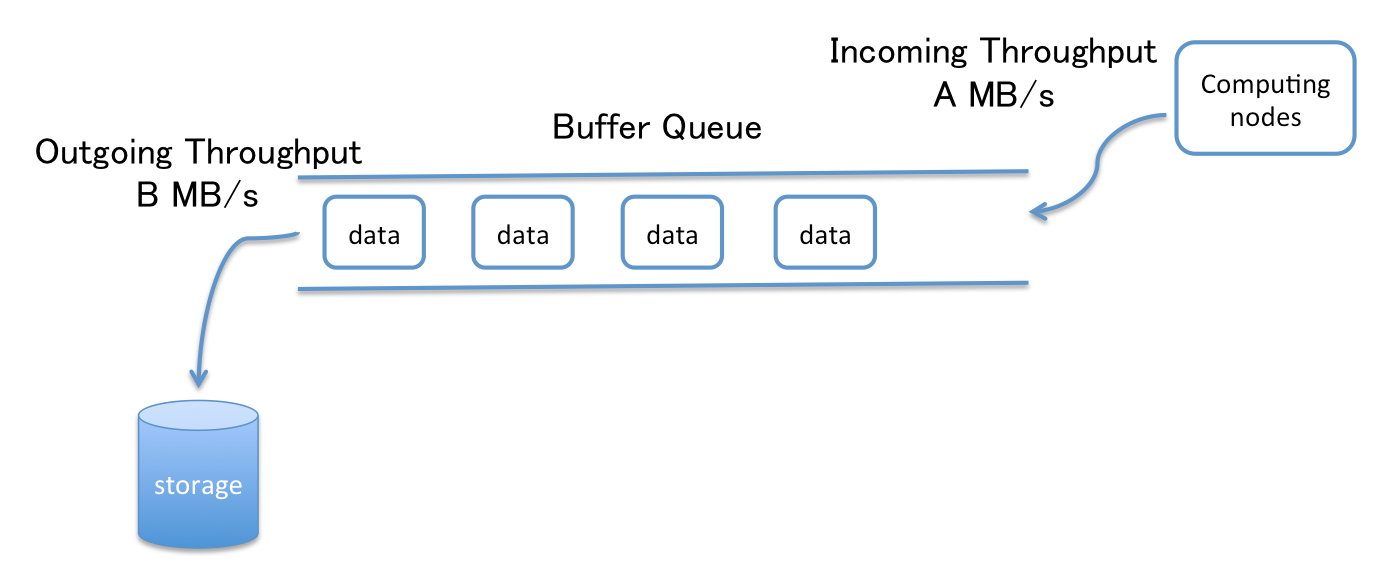
\includegraphics[width=6cm]{../img/buffer_queue}
	\caption{buffer queue}
	\label{buffer queue}
\end{figure}

If the buffer size is unlimited. then we can buffer all data in the I/O buffer nodes, and achieve a high throughput in cloud burst \kento{Good work !! As I said in the different sections, it's important to remind its motivation before describing the algorithm, techniques, model, or methods for its reminder}.
However buffer size can not be unlimited, we can not buffer all data in the I/O buffer nodes, data in buffer nodes have to be write back to storage in another system.
The problem is which data should be written back to storage, like cache in cpu, if we can reduce cache miss in this situation, we can increase throughput. 
According to data locality, we use a priority queue to determine which data should be write back.

Consider Fig.~\ref{buffer queue}, assume average incoming throughput is A MB/s and average outgoing throughput is B MB/s, if A always larger than B, after $T$ time buffer queue will full.
\[T=\frac{m_2\times n_2}{A-B}\]

After that, since buffer queue is full, I/O server can not send more data to I/O buffer nodes, have to block any read and write request since that.
In this case, jobs running on public cloud have to be moved back to original system until buffer queue is empty
\kento{Why ??}.
